\chapter{Methods}
\label{chapterlabel3}

The method of tackling this problem will be based on previous research done in this domain. There are three essential components for this project:
\begin{figure}[h]
\caption{Basic flowchart}
\centering
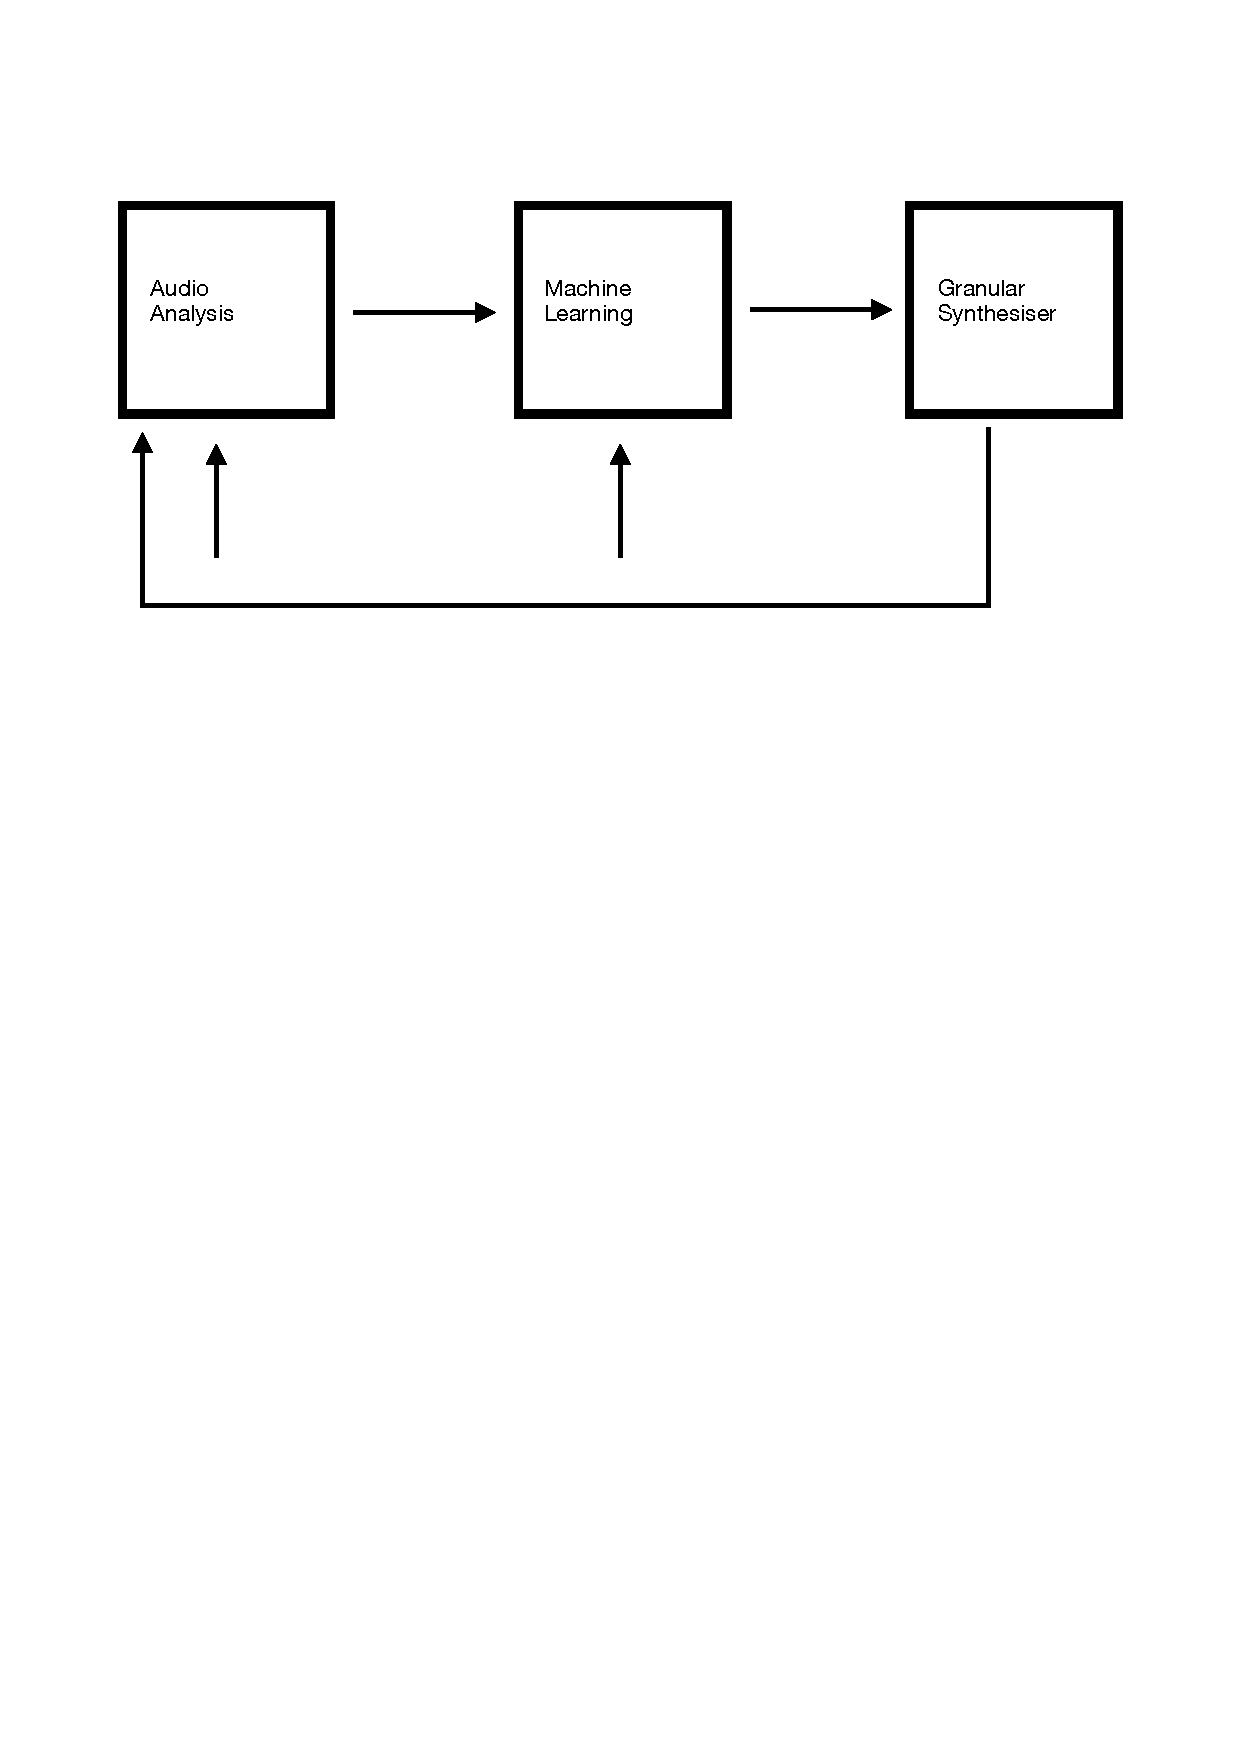
\includegraphics[width=0.5\textwidth]{images/flowchart}
\end{figure}

The box ``Granular Synthesiser'' in figure 1. represents a granular synthesizer.
It will be build in C++, using openFrameworks and the Maximillian
% \cite{micknoise_c++_2019}
library.

``Machine Learning'' in figure 1, stands for Machine Learning. This aspect will
most likely be implemented in python, either using the
``scikit.learn''
%\cite{noauthor_scikit-learn:_nodate}
library, or the
``TensorFlow''
% \cite{noauthor_tensorflow_nodate}
library. Depending on which
Machine Learning algorithms will be used. This will be determined during
testing. The ones being considered at the moment include k-NN, Neural Networks,
and LSTM(Long Short-Term Memory Neural Network)
%\cite{yee-king_automatic_2018}.

The ``Audio Analysis'' box in figure 1. represents the aspect of the project responsible for extracting audio features from input sounds. This requires some testing in order to see which works best for this task. Feature extractors considered are: MFCC and DBM. Environment choices for now include the python ``pyAudioAnalysis'' for Python, and ``Essentia'' library for C++.

Training of whichever algorithm chosen will be happening on data generated by
me. Vectors of synthesis engine parameter values, and audio analysis values,
possibly as a CSV file will be created. The goal here is to automate a sampled
walk through the parameter space, and extract audio features for each point.
This was suggested to me by Dr. Rebecca Fiebrink, during her office hours, as
part of feedback for another assignment. Possibly,  a genetic algorithm could be
used for this process
%\cite{yee-king_automatic_2018}.

Once all the pieces are working, the key thing is to make them all work together as soon as possible, to create a working prototype, from which, by user testing and iterative design I can move forward and improve the project tackling issues one by one.

The minimum viable prototype has to include every aspect from Figure 1., excluding any substantial testing. Meaning, that one audio feature extractor, one machine learning algorithm, and a synthesizer that work together would be enough. Any testing of possibilities, whether audio feature extractors, or machine learning algorithms is outside of the scope of a prototype. As long as each piece of software can communicate and produce a desirable end result, the prototype will be considered successful.














\iffalse
 What belongs in the "methods" section of a scientific paper?

    Information to allow the reader to assess the believability of your results.
    Information needed by another researcher to replicate your experiment.
    Description of your materials, procedure, theory.
    Calculations, technique, procedure, equipment, and calibration plots. 
    Limitations, assumptions, and range of validity.
    Desciption of your analystical methods, including reference to any specialized statistical software. 

The methods section should answering the following questions and caveats: 

    Could one accurately replicate the study (for example, all of the optional and adjustable parameters on any sensors or instruments that were used to acquire the data)?
    Could another researcher accurately find and reoccupy the sampling stations or track lines?
    Is there enough information provided about any instruments used so that a functionally equivalent instrument could be used to repeat the experiment?
    If the data are in the public domain, could another researcher lay his or her hands on the identical data set?
    Could one replicate any laboratory analyses that were used? 
    Could one replicate any statistical analyses?
    Could another researcher approximately replicate the key algorithms of any computer software?

Citations in this section should be limited to data sources and references of where to find more complete descriptions of procedures.
Do not include descriptions of results. 
\fi